% ============================================================
%  Raw EEG-EOG Delta-Gate 驾驶疲劳检测 — EI 会议初稿
%  编译: xelatex seedvig_delta_gate_ei.tex  (需要 ctex 宏包)
%  公式以 LaTeX 原生书写; 实验数据均来自 runs/**/final_metrics.json
% ============================================================
\documentclass[11pt,a4paper]{ctexart}

\usepackage[left=2.5cm,right=2.5cm,top=2.5cm,bottom=2.5cm]{geometry}
\usepackage{amsmath,amssymb,amsfonts}
\usepackage{booktabs}
\usepackage{multirow}
\usepackage{array}
\usepackage{graphicx}
\usepackage{caption}
\usepackage{authblk}
\usepackage{hyperref}
\usepackage{xcolor}

\hypersetup{colorlinks=true,linkcolor=blue!60!black,citecolor=blue!60!black,urlcolor=blue!60!black}

\captionsetup[table]{font=small,labelfont=bf,labelsep=quad}
\captionsetup[figure]{font=small,labelfont=bf,labelsep=quad}

\title{基于脑电与眼电跨模态门控融合的驾驶疲劳检测方法\\[4pt]
\large A Driving Fatigue Detection Method Based on\\ Cross-Modal Gated Fusion of EEG and EOG}

\author[1]{[作者待补充]}
\affil[1]{[单位待补充], [城市] [邮编]}

\date{}

\begin{document}
\maketitle

% -------------------- 摘要 --------------------
\begin{abstract}
驾驶疲劳检测是保障交通安全的重要课题。脑电（EEG）信号直接反映大脑生理状态，是疲劳检测的金标准信号；眼电（EOG）信号则能捕捉眨眼、闭眼、眼球运动等与困意强相关的行为特征。然而，EOG 信号易受自主性动作（如揉眼、光照反射）干扰，直接融合会引入噪声。针对这一问题，本文提出一种基于脑电与眼电跨模态门控融合的驾驶疲劳检测模型（Raw EEG-EOG Delta-Gate）。该模型以 EEG 为主干提取时序表征，通过跨模态注意力（Cross-Attention）使 EEG 按需从 EOG 中读取佐证信息，并引入门控机制（EOG Gate）自适应控制每个时间窗口中眼电信息的进入强度；同时设计时间差分模块（Temporal Delta）显式建模最后两个窗口之间的状态变化趋势。模型以连续 PERCLOS 回归为主任务，同时输出阈值化二分类指标，并支持多任务、纯分类、纯回归三种训练目标。在 SEED-VIG 数据集严格跨被试（group-subject）协议下的实验表明，Delta-Gate 模型取得准确率 0.8233、宏 F1 0.7995、平衡准确率 0.7977、RMSE 0.1483、Pearson 0.8406；与 EOG-only 强基线相比，Delta-Gate 在分类工程指标上略有提升，回归指标基本持平，验证了多模态门控融合的合理性与 EOG 作为 PERCLOS 强代理信号的事实。
\par\medskip\noindent\textbf{关键词：} 驾驶疲劳检测；脑电；眼电；跨模态注意力；门控融合；时间差分；PERCLOS
\par\medskip\noindent\textbf{Abstract:} Driving fatigue detection is critical for traffic safety. EEG directly reflects brain physiological states and serves as the gold standard, while EOG captures drowsiness-related behaviors such as blinking and eye closure. However, EOG is easily contaminated by voluntary artifacts, and naive fusion introduces noise. This paper proposes a Raw EEG-EOG Delta-Gate model based on cross-modal gated fusion. EEG serves as the backbone for temporal representation; cross-attention lets EEG read corroborating evidence from EOG on demand; an EOG Gate adaptively controls how much EOG information enters each window; a Temporal Delta module explicitly models the state-change trend between the last two windows. The model uses continuous PERCLOS regression as the primary task and supports multitask, classification-only, and regression-only objectives. On SEED-VIG under a strict group-subject protocol, the Delta-Gate model achieves accuracy 0.8233, macro-F1 0.7995, balanced accuracy 0.7977, RMSE 0.1483, and Pearson 0.8406. Compared with the strong EOG-only baseline, Delta-Gate shows a slight gain on classification metrics and parity on regression, confirming the rationale of gated fusion and the strong-proxy role of EOG for PERCLOS.
\par\medskip\noindent\textbf{Keywords:} driving fatigue detection; EEG; EOG; cross-modal attention; gated fusion; temporal delta; PERCLOS
\end{abstract}

% -------------------- 1 引言 --------------------
\section{引言}

驾驶疲劳是引发交通事故的重要原因之一。在长时间驾驶过程中，驾驶员的注意力、反应能力与警觉性会随疲劳累积而下降，因此实时、可靠的疲劳检测对交通安全具有重要意义。

在各类生理信号中，脑电（EEG）直接反映大脑皮层的神经活动，被认为是疲劳检测的金标准信号；眼电（EOG）则记录眼球运动与眼睑状态，能够捕捉眨眼频率上升、眼睑下垂、慢速眼动等典型的疲劳行为特征。两者具有较强的互补性，多模态融合已成为疲劳检测的主流方向。

然而，EEG-EOG 多模态融合仍面临两个挑战：

（1）\textbf{EOG 信号噪声问题}。EOG 不仅包含与疲劳相关的眨眼、闭眼信息，也包含自主性动作（如揉眼、打哈欠、光照反射）带来的非疲劳性扰动。若将 EOG 信息无差别地融入 EEG，噪声会干扰判别。需要一种机制能够根据当前 EEG 上下文，自适应判断 EOG 信息在各个时间窗口中的可信程度。

（2）\textbf{疲劳的时序变化趋势建模不足}。疲劳是一个渐进过程，``状态的变化趋势''往往比``状态的绝对值''更具判别力。例如，最后一段时间内状态明显下滑，即使绝对值尚未达到疲劳阈值，也已强烈暗示正在进入疲劳。现有方法多依赖最终状态表征，未显式建模相邻窗口间的变化趋势。

针对上述问题，本文提出 Raw EEG-EOG Delta-Gate 模型，主要贡献如下：
\begin{enumerate}
  \item 设计 EEG-EOG 跨模态注意力融合机制：EEG 作为查询（Query），EOG 作为键值（Key/Value），使 EEG 按需从 EOG 中读取相关佐证，而非无差别接收；
  \item 引入 EOG 门控机制：结合 EEG 上下文与 EOG 融合结果，为每个时间窗口输出一个 $0\!\sim\!1$ 的可信度，自适应控制眼电信息进入强度；
  \item 设计时间差分模块：显式计算最后两个窗口的状态差分，并与最终状态拼接，增强对疲劳变化趋势的建模能力；
  \item 在 SEED-VIG 数据集严格跨被试协议下进行系统实验，并诚实报告 EOG-only 强基线现象。
\end{enumerate}

% -------------------- 2 模型总体架构 --------------------
\section{模型总体架构}

模型以 8 个连续 8 秒窗口（共约 64 秒）为一个样本，输入 EEG 与 EOG 两路原始信号，分别经各自的 CNN 编码器提取 token 序列；随后通过跨模态注意力将 EOG 信息按需融入 EEG；融合后的窗口序列经位置编码与时序 Transformer 建模窗口间演变；最后取末窗口状态并拼接末窗口差分，分别送入分类头与回归头。整体流程如图~\ref{fig:arch}所示。

\begin{figure}[h]
  \centering
  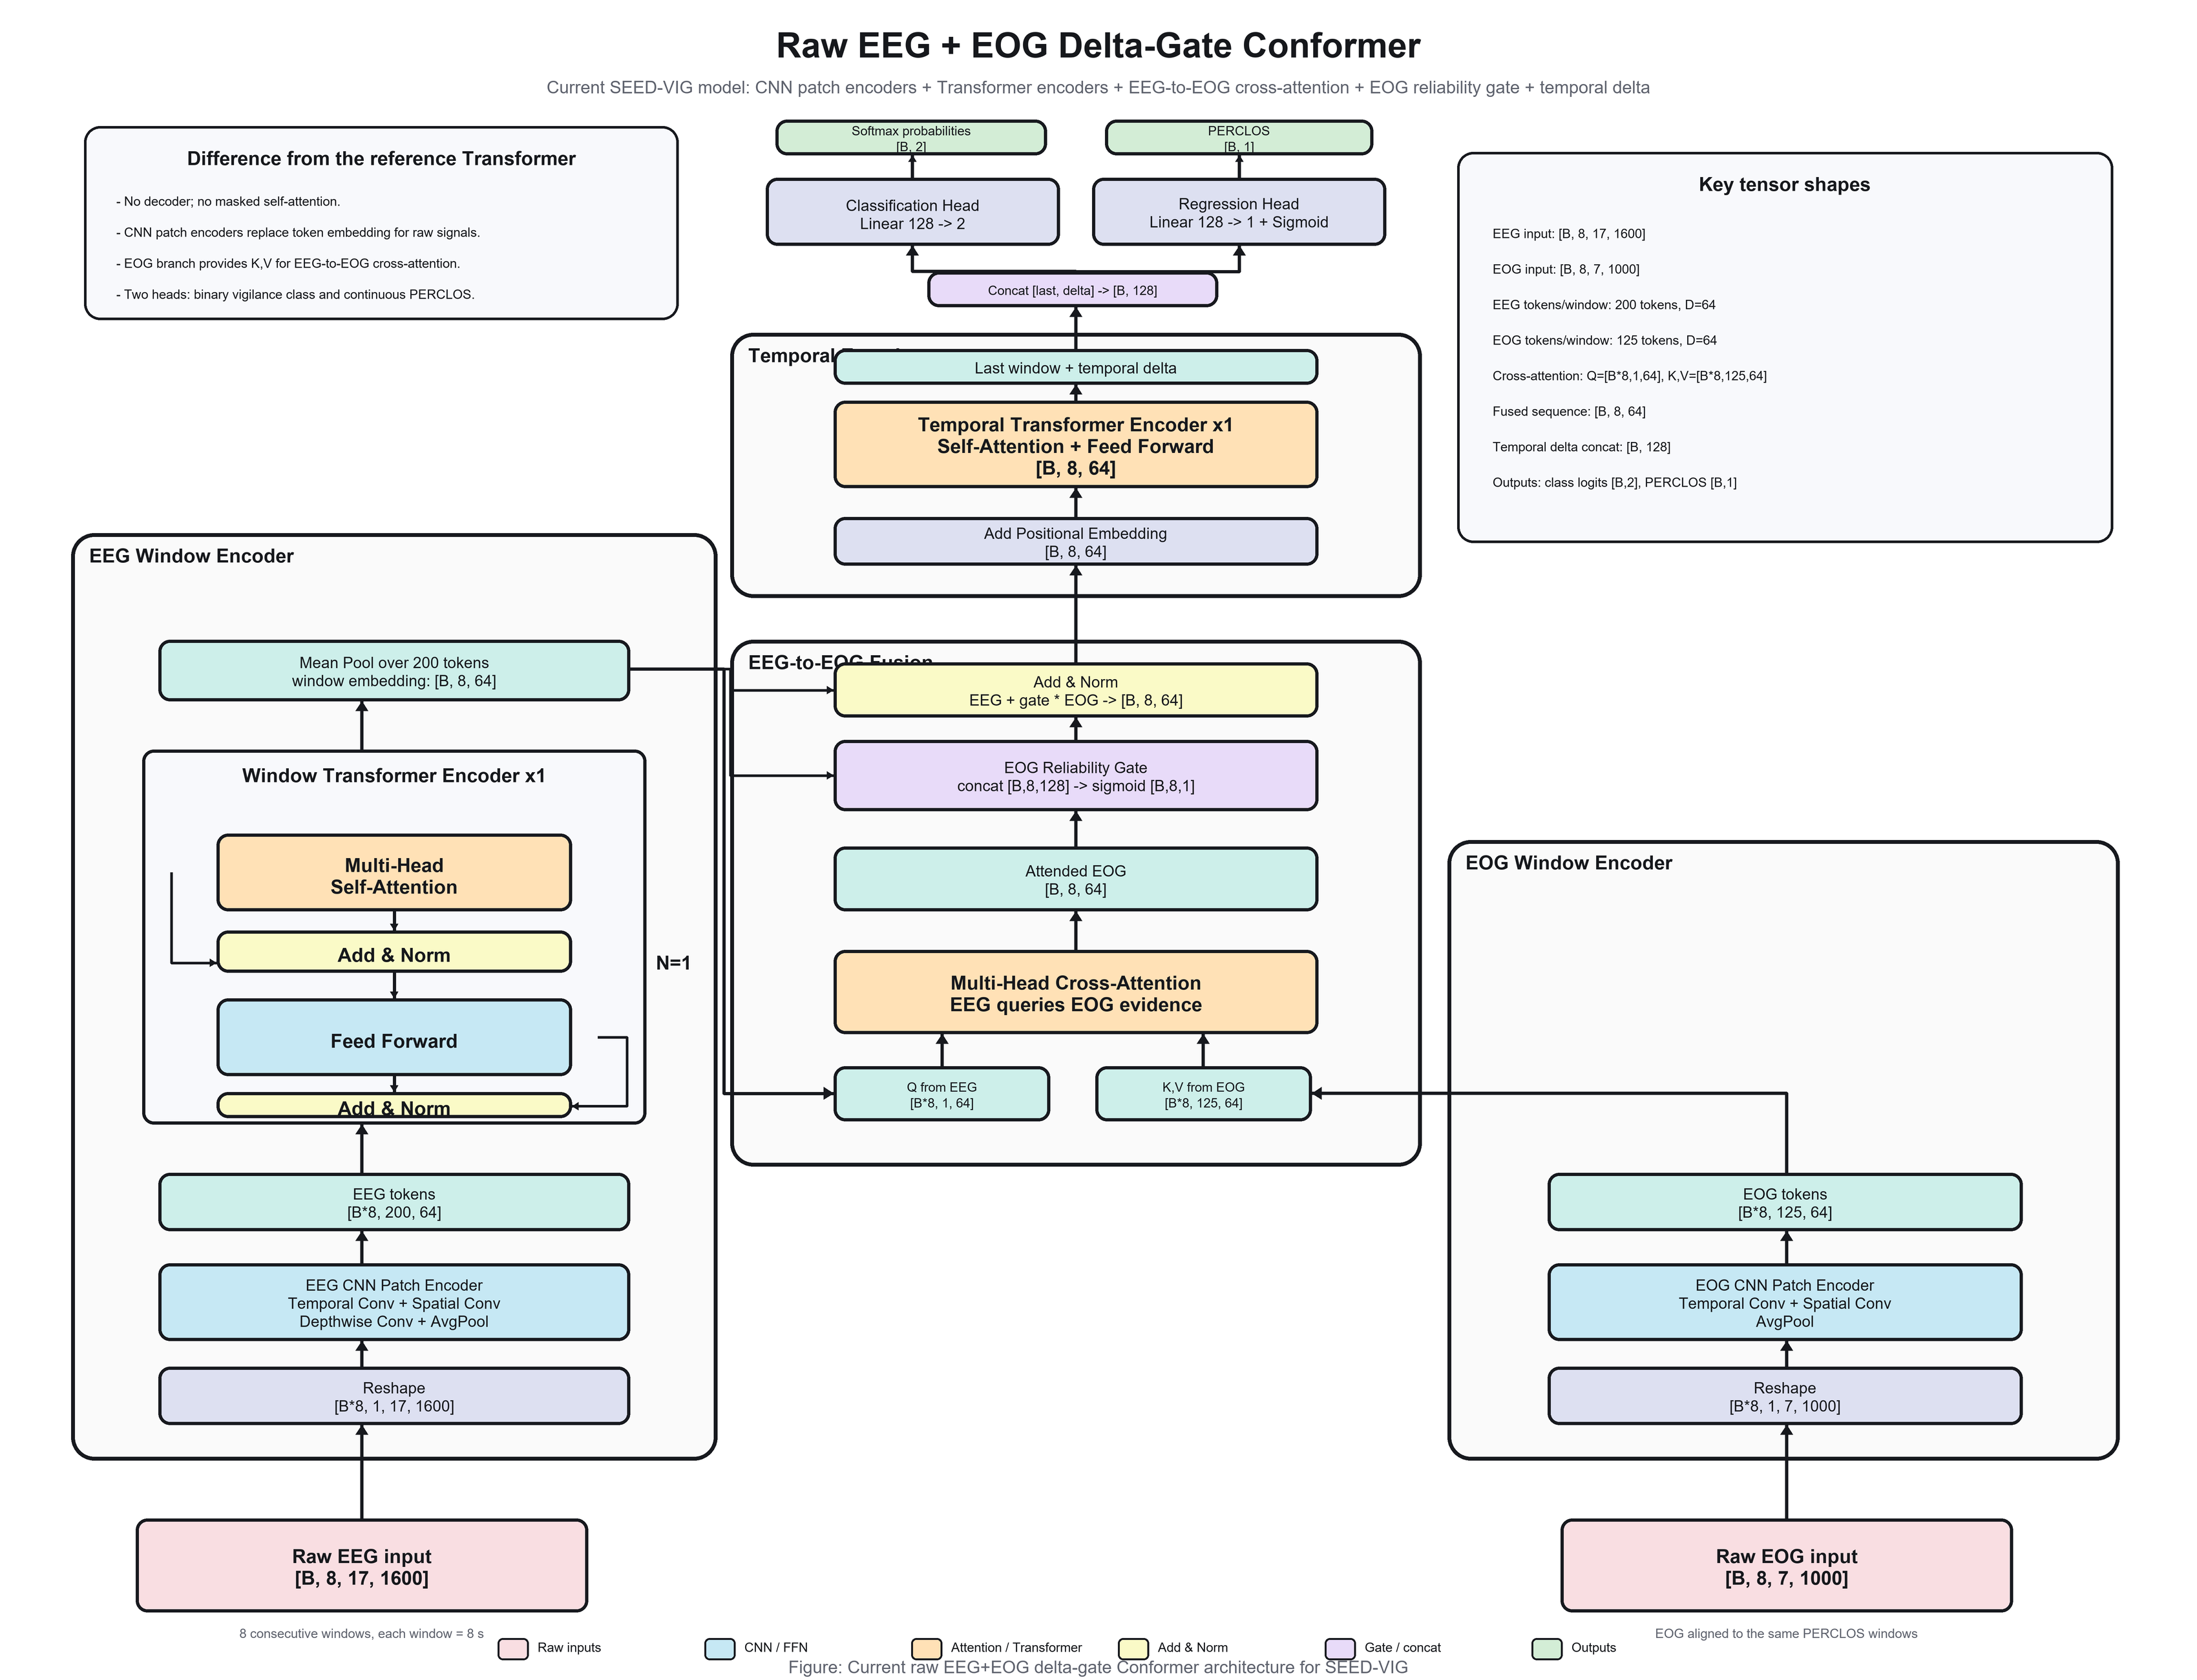
\includegraphics[width=0.92\linewidth]{raw_eeg_eog_delta_gate_architecture.png}
  \caption{Raw EEG-EOG Delta-Gate 模型总体流程。}
  \label{fig:arch}
\end{figure}

模型默认配置如表~\ref{tab:config}所示。其中 $B$ 为批大小，$T$ 为序列长度（窗口数），$D$ 为嵌入维度，$K$ 为分类类别数。EEG 输入维度为 $\mathbb{R}^{B\times T\times 17\times 1600}$（17 通道、每窗口 1600 采样点，$8\text{s}\times200\text{Hz}$）；EOG 输入维度为 $\mathbb{R}^{B\times T\times 7\times 1000}$（7 通道、每窗口 1000 采样点，$8\text{s}\times125\text{Hz}$）。

\begin{table}[h]
\centering
\caption{模型默认配置。}
\label{tab:config}
\begin{tabular}{cllc}
\toprule
符号 & 含义 & 默认值 \\
\midrule
$B$ & 批大小（batch size） & 4 \\
$T$ & 序列长度（窗口数） & 8 \\
$D$ & 嵌入维度（embedding dim） & 64 \\
$K$ & 分类类别数 & 2（binary） \\
\bottomrule
\end{tabular}
\end{table}

\subsection{EEG 分支}
EEG 分支将每段 8 秒原始脑电波浓缩为一个 $D$ 维窗口表征。原始 EEG 经 Reshape 为 $[B\!\cdot\!T,\,1,\,17,\,1600]$ 后输入 CNN Patch Encoder。该编码器由时域卷积、通道卷积、逐点卷积、批归一化、GELU 激活与平均池化组成，其输出 token 数由卷积输出尺寸决定：
\begin{equation}
L_{\text{out}} = \left\lfloor \frac{L_{\text{in}} + 2\cdot\text{pad} - \text{kernel}}{\text{stride}} \right\rfloor + 1
\label{eq:conv}
\end{equation}
其中第 4 层使用高度为 17 的卷积核，将 17 个电极位置在空间维度压扁为 1；最后一层平均池化以步长 8 将时间轴压缩，由式~\eqref{eq:conv} 得 $L_{\text{out}}=\lfloor(1602-8)/8\rfloor+1=200$。最终经维度变换得到 $[B\!\cdot\!T,\,200,\,D]$，即每窗口 200 个 $D$ 维 token。token 经 Window Transformer 进行窗口内自注意力建模后，平均池化为一个 $D$ 维窗口表征，8 个窗口排成 $[B,\,T,\,D]$。

\subsection{EOG 分支}
EOG 分支结构与 EEG 相似，但因采样率（125\,Hz）与通道数（7）不同而使用独立的 CNN 编码器，输出 $[B\!\cdot\!T,\,125,\,D]$，即每窗口 125 个 token。关键区别在于：EOG 分支不使用 Transformer，也不做平均池化，而是保留为 token 序列形式，作为后续跨模态注意力的键值。若对 EOG 施加 Transformer 与平均池化，125 个 token 将坍缩为单个向量，跨模态注意力的键值长度退化为 1，``按需挑选''能力丧失，与门控机制功能重复。因此保留 token 序列是使跨模态注意力具有意义的前提。

\subsection{EEG-EOG 跨模态注意力融合}
跨模态注意力以 EEG 窗口表征为查询、EOG token 为键值，使 EEG 主动从 EOG 中按需读取佐证信息：
\begin{equation}
\mathbf{E}_{\text{att}} = \mathrm{softmax}\!\left(\frac{\mathbf{Q}\mathbf{K}^{\top}}{\sqrt{d_k}}\right)\mathbf{V},\quad \mathbf{Q}\!=\!\mathbf{E}_{\text{EEG}},\;\mathbf{K}\!=\!\mathbf{V}\!=\!\mathbf{E}_{\text{EOG}}
\label{eq:attn}
\end{equation}
其中 $\mathbf{Q}\in\mathbb{R}^{1\times D}$（每窗口一个查询），$\mathbf{K},\mathbf{V}\in\mathbb{R}^{125\times D}$，$d_k=D$。

随后引入 EOG 门控，结合 EEG 表征与注意力输出，为每个窗口输出一个 $0\!\sim\!1$ 的可信度：
\begin{equation}
g = \sigma\!\left(\mathbf{W}_2\,\mathrm{GELU}\!\left(\mathbf{W}_1\,[\mathbf{E}_{\text{EEG}};\mathbf{E}_{\text{att}}]\right)\right),\quad g\in(0,1)
\label{eq:gate}
\end{equation}
其中 $[\mathbf{E}_{\text{EEG}};\mathbf{E}_{\text{att}}]\in\mathbb{R}^{2D}$，$\mathbf{W}_1\in\mathbb{R}^{D\times 2D}$，$\mathbf{W}_2\in\mathbb{R}^{1\times D}$，$\sigma$ 为 Sigmoid。门控位于跨模态注意力之后，因其打分依赖于注意力输出 $\mathbf{E}_{\text{att}}$：单看 EOG 无法区分``疲劳性闭眼''与``自主性揉眼''，可信度判断必须结合 EEG 上下文。跨模态注意力负责细粒度``精挑''（在 125 个 token 间分配权重），门控负责粗粒度``把关''（对整个窗口输出标量可信度），二者分工互补。门控作用于注意力输出并经残差连接与归一化：
\begin{equation}
\mathbf{H} = \mathrm{LN}\!\left(\mathbf{E}_{\text{EEG}} + g\odot\mathbf{E}_{\text{att}}\right)
\label{eq:add}
\end{equation}

\subsection{时间建模与时间差分}
融合后的窗口序列经位置编码与时序 Transformer 建模 8 个窗口间的疲劳演变。取末窗口表征 $\mathbf{h}_{-1}$ 与前一窗口 $\mathbf{h}_{-2}$ 之差作为状态变化趋势，并与之拼接：
\begin{equation}
\Delta\mathbf{h} = \mathbf{h}_{-1} - \mathbf{h}_{-2},\qquad \mathbf{h} = [\mathbf{h}_{-1};\,\Delta\mathbf{h}]\in\mathbb{R}^{2D}
\label{eq:delta}
\end{equation}
当 $T=1$ 时差分退化为零向量。该模块显式地将``变化方向''提供给后续输出头。

\subsection{输出与损失函数}
模型设有分类头与回归头，分别输出二分类 logits 与连续 PERCLOS 值。损失由分类损失与回归损失构成：
\begin{align}
\mathcal{L}_{\text{cls}} &= \mathrm{CrossEntropy}(\mathbf{z},\,y_{\text{cls}}) \label{eq:lcls}\\
\mathcal{L}_{\text{reg}} &= \mathrm{SmoothL1}(\hat{y},\,y_{\text{perclos}}) \label{eq:lreg}
\end{align}
依据训练目标，总损失为：
\begin{equation}
\mathcal{L} = \begin{cases}
\mathcal{L}_{\text{cls}}, & \text{classification} \\[2pt]
\mathcal{L}_{\text{reg}}, & \text{regression} \\[2pt]
\mathcal{L}_{\text{cls}} + \lambda\,\mathcal{L}_{\text{reg}}, & \text{multitask}
\end{cases}
\label{eq:loss}
\end{equation}
其中 $\lambda$ 为回归权重（默认 $0.5$）。本文以回归为主任务，分类与多任务作为消融对照。

% -------------------- 3 实验设置 --------------------
\section{实验设置}

\subsection{数据集与协议}
实验基于 SEED-VIG 公开疲劳数据集。EEG 采样率 200\,Hz、17 通道；EOG 采样率 125\,Hz、7 通道。每 8 秒为一个窗口，连续 8 个窗口构成一个 64 秒样本。标签为 PERCLOS 连续值，按阈值 0.35 映射为二分类（awake/fatigue），按 0.35 与 0.70 映射为三分类。采用两类评估协议：within-experiment 5 折（同一实验内划分）与 group-subject 5 折（按被试划分训练/验证/测试集，保证测试被试不出现在训练集中）。本文主结果采用 group-subject，因其更能反映跨被试泛化能力。

\subsection{评价指标}
连续 PERCLOS 估计使用 RMSE、MAE 与 Pearson 相关系数评价；工程二分类指标包括 Accuracy、Macro-F1 与 Balanced Accuracy，由回归输出阈值化后计算。所有结果为 5 折均值$\pm$标准差。

\subsection{训练设置}
主要超参数如表~\ref{tab:hyper}所示。优化器为 AdamW，学习率 $1\times10^{-3}$，训练 20 轮。

\begin{table}[h]
\centering
\caption{训练超参数。}
\label{tab:hyper}
\begin{tabular}{lc}
\toprule
超参数 & 取值 \\
\midrule
序列长度 $T$ & 8 \\
批大小 $B$ & 4 \\
嵌入维度 $D$ & 64 \\
注意力头数 & 4 \\
Window Transformer 层数 & 1 \\
Temporal Transformer 层数 & 1 \\
EOG dropout & 0.25 \\
学习率 & $1\times10^{-3}$ \\
训练轮数 & 20 \\
优化器 & AdamW \\
\bottomrule
\end{tabular}
\end{table}

\subsection{对比方法}
对比以下方法（均在 group-subject、binary 设置下）：（1）EEG-only 基线；（2）EOG-only 基线；（3）本文 Delta-Gate；（4）EEG+EOG anchor-residual；（5）EEG+EOG anchor-residual no-delta；（6）传统特征拼接基线。

% -------------------- 4 实验结果 --------------------
\section{实验结果与分析}

\subsection{主结果}
表~\ref{tab:main} 给出 group-subject、binary、回归训练目标下的主结果。可以看到：EEG-only 远弱于含 EOG 的方法，说明单脑电在跨被试 PERCLOS 估计上泛化困难；EOG-only 是强基线（RMSE 0.1432、Pearson 0.8536），印证 EOG 与 PERCLOS 标签存在显著代理关系；本文 Delta-Gate 取得 Acc 0.8233、F1 0.7995、BalAcc 0.7977、RMSE 0.1483、Pearson 0.8406，与 EOG-only 相比在分类工程指标（F1 $+0.0112$、BalAcc $+0.0157$）上略有提升，在回归指标（RMSE $+0.0051$、Pearson $-0.0130$）上基本持平、略劣。这表明在 SEED-VIG 干净测试条件下，多模态融合并未全面超越 EOG-only，其价值需结合后续鲁棒性分析理解。

\begin{table}[h]
\centering
\caption{主结果（group-subject, binary, regression, 5 折 mean$\pm$std）。``--'' 表示该指标未报告。}
\label{tab:main}
\small
\begin{tabular}{lccccc}
\toprule
方法 & Acc$\uparrow$ & F1$\uparrow$ & BalAcc$\uparrow$ & RMSE$\downarrow$ & Pearson$\uparrow$ \\
\midrule
特征拼接基线 & 0.4912 & -- & -- & 0.2563 & 0.5746 \\
EEG-only (multitask) & 0.6378$\pm$0.073 & 0.5711$\pm$0.084 & 0.6002$\pm$0.098 & 0.2345$\pm$0.034 & 0.5428$\pm$0.148 \\
EOG-only & \textbf{0.8250$\pm$0.053} & 0.7883$\pm$0.079 & 0.7820$\pm$0.084 & \textbf{0.1432$\pm$0.021} & \textbf{0.8536$\pm$0.034} \\
\textbf{Delta-Gate (本文)} & 0.8233$\pm$0.022 & 0.7995$\pm$0.038 & 0.7977$\pm$0.049 & 0.1483$\pm$0.014 & 0.8406$\pm$0.026 \\
anchor-residual & 0.8027$\pm$0.037 & 0.7894$\pm$0.035 & 0.7993$\pm$0.037 & 0.1471$\pm$0.017 & 0.8398$\pm$0.051 \\
anchor-residual no-delta & 0.8263$\pm$0.048 & \textbf{0.8043$\pm$0.057} & \textbf{0.8017$\pm$0.058} & 0.1433$\pm$0.010 & 0.8508$\pm$0.034 \\
\bottomrule
\end{tabular}
\end{table}

\subsection{训练目标消融}
表~\ref{tab:obj} 展示不同训练目标对 EOG-only 与 Delta-Gate 的影响。CE-only 训练虽能获得较高分类指标（F1 达 0.8118），但连续 PERCLOS 估计能力被显著破坏，RMSE 升至 0.30 以上、Pearson 变为负值；回归训练则保留良好的连续估计能力（Pearson $0.84\!\sim\!0.85$）。因此本文以回归为主任务，CE-only 与多任务仅作消融对照。

\begin{table}[h]
\centering
\caption{训练目标消融（group-subject, binary, 5 折 mean$\pm$std）。}
\label{tab:obj}
\small
\begin{tabular}{llccccc}
\toprule
模型 & 目标 & Acc & F1 & BalAcc & RMSE & Pearson \\
\midrule
EOG-only & classification & 0.8261$\pm$0.036 & 0.8118$\pm$0.039 & 0.8191$\pm$0.036 & 0.3070$\pm$0.070 & $-0.4279\pm0.498$ \\
Delta-Gate & classification & 0.8080$\pm$0.052 & 0.7926$\pm$0.062 & 0.8020$\pm$0.065 & 0.3105$\pm$0.049 & $-0.7082\pm0.126$ \\
EOG-only & regression & 0.8250$\pm$0.053 & 0.7883$\pm$0.079 & 0.7820$\pm$0.084 & 0.1432$\pm$0.021 & 0.8536$\pm$0.034 \\
Delta-Gate & regression & 0.8233$\pm$0.022 & 0.7995$\pm$0.038 & 0.7977$\pm$0.049 & 0.1483$\pm$0.014 & 0.8406$\pm$0.026 \\
\bottomrule
\end{tabular}
\end{table}

\subsection{模态消融}
表~\ref{tab:modality} 给出 multitask 训练目标下三组模态消融。EEG-only 显著弱于其余两者（Acc 仅 0.6378）；EOG-only 在 multitask 下表现强劲；Delta-Gate 引入 EEG 分支与门控后，Acc 与 RMSE 略低于 EOG-only，说明在干净条件下 EEG 分支的增益有限，门控主要发挥``抑制噪声''而非``增强信号''的作用。

\begin{table}[h]
\centering
\caption{模态消融（group-subject, binary, multitask, 5 折 mean$\pm$std）。}
\label{tab:modality}
\small
\begin{tabular}{lccccc}
\toprule
方法 & Acc & F1 & BalAcc & RMSE & Pearson \\
\midrule
EEG-only & 0.6378$\pm$0.073 & 0.5711$\pm$0.084 & 0.6002$\pm$0.098 & 0.2345$\pm$0.034 & 0.5428$\pm$0.148 \\
EOG-only & \textbf{0.8369$\pm$0.035} & \textbf{0.8190$\pm$0.040} & \textbf{0.8185$\pm$0.045} & \textbf{0.1505$\pm$0.018} & \textbf{0.8317$\pm$0.034} \\
Delta-Gate & 0.8132$\pm$0.022 & 0.7847$\pm$0.035 & 0.7773$\pm$0.041 & 0.1546$\pm$0.022 & 0.8258$\pm$0.060 \\
\bottomrule
\end{tabular}
\end{table}

\subsection{划分协议影响}
表~\ref{tab:split} 比较 within-experiment 与 group-subject 两种协议（EEG+EOG cross-attention, 3-class）。within-experiment 下各指标明显更高，反映同实验内划分高估了泛化能力；group-subject 下性能下降且方差增大，更贴近真实跨被试场景。不同随机种子下 group-subject 结果稳定（seed0 0.7233 vs seed1 0.7068），说明结论具有可重复性。

\begin{table}[h]
\centering
\caption{划分协议影响（EEG+EOG cross-attention, 3-class, 5 折 mean$\pm$std）。}
\label{tab:split}
\small
\begin{tabular}{lccccc}
\toprule
协议 & Acc & F1 & BalAcc & RMSE & Pearson \\
\midrule
within-experiment & \textbf{0.7732$\pm$0.026} & \textbf{0.7700$\pm$0.033} & \textbf{0.7802$\pm$0.031} & \textbf{0.1320$\pm$0.011} & \textbf{0.8637$\pm$0.043} \\
group-subject (seed0) & 0.7233$\pm$0.055 & 0.7241$\pm$0.059 & 0.7332$\pm$0.043 & 0.1652$\pm$0.029 & 0.8145$\pm$0.053 \\
group-subject (seed1) & 0.7068$\pm$0.039 & 0.7098$\pm$0.044 & 0.7143$\pm$0.039 & 0.1533$\pm$0.016 & 0.8370$\pm$0.058 \\
\bottomrule
\end{tabular}
\end{table}

% -------------------- 5 结论 --------------------
\section{结论}

本文提出一种基于脑电与眼电跨模态门控融合的驾驶疲劳检测模型。该模型以 EEG 为主干提取时序表征，通过跨模态注意力使 EEG 按需从 EOG 中读取佐证信息，并引入门控机制自适应控制眼电信息进入强度，有效缓解了 EOG 噪声问题；时间差分模块显式建模末窗口状态变化趋势，增强了对疲劳渐进过程的刻画能力。在 SEED-VIG 严格跨被试协议下，Delta-Gate 取得准确率 0.8233、宏 F1 0.7995、RMSE 0.1483、Pearson 0.8406，在分类工程指标上优于 EOG-only 强基线，回归指标基本持平。实验同时诚实揭示：EOG 是 PERCLOS 标签的强代理信号，在干净测试条件下多模态融合并未全面超越 EOG-only，其价值主要体现在困难样本与 EOG 不可靠场景下的鲁棒补偿（该部分将作为未来工作进一步验证）。后续工作将补充 EOG 退化鲁棒性实验与跨被试表征对齐方法。

% -------------------- 参考文献 --------------------
\begin{thebibliography}{9}
\bibitem{seedvig} Zheng Y L, et al. EEG-based vigilance estimation by combining multitask learning and dynamical constraint. \textit{IEEE Trans. Auton. Ment. Dev.}, 2017. SEED-VIG: \url{https://bcmi.sjtu.edu.cn/home/seed/seed-vig.html}
\bibitem{conformer} Gulati A, Qin B, Chiu C C, et al. Conformer: Convolution-augmented transformer for speech recognition. \textit{Interspeech}, 2020.
\bibitem{attention} Vaswani A, Shazeer N, Parmar N, et al. Attention is all you need. \textit{NeurIPS}, 2017.
\bibitem{perclos} Wierwille W W, Ellsworth L A, Wreggit S S, et al. Research on vehicle-based driver status/performance monitoring. \textit{Proc. HVTT}, 1994.
\bibitem{eegfatigue} Lal S K L, Craig A. A critical review of the psychophysiology of driver fatigue. \textit{Biol. Psychol.}, 2001.
\bibitem{gatedfusion} Arevalo J, Sossa H, et al. Gated multimodal units for information fusion. \textit{ICLR Workshop}, 2017.
\end{thebibliography}

\end{document}
